\documentclass[a4paper,8pt]{article}

\usepackage[utf8]{inputenc}
\usepackage[spanish]{babel}
\usepackage{enumerate}
\usepackage{graphicx}
\usepackage{array}
\usepackage{colortbl}
\usepackage{hyperref}
\usepackage[hyperpageref]{backref}
\usepackage{calc}
\usepackage{fancyhdr}
\usepackage{lastpage}
\usepackage{geometry}
\usepackage{todonotes}
\usepackage{todonotes}
\usepackage{amsmath}
\usepackage{multirow}
\usepackage{arydshln}
\usepackage{color,soul}
\usepackage[normalem]{ulem}

\geometry{
  inner=30mm,
  outer=25mm,
  top=35mm,
  bottom=30mm,
  marginpar=20mm, reversemp
}


\newcommand{\paperindex}{$\mathcal{OC}$}
\newcommand{\sinc}{{\color{blue}s}inc(\textit{\color{red}i})}

\begin{document}

\begin{titlepage}
	\centering	
	{\scshape\large PROPUESTA DE TESIS DOCTORAL \par}
	\vspace{2cm}
	{\Large\bfseries \'Indices para validaci\'on de algoritmos de clustering\par}
	\vspace{1.5cm}
	{\Large\itshape David N. Campo \par}
	\vspace{2cm}
	{\normalsize Instituto de Investigación de Señales, Sistemas e Inteligencia Computacional (\sinc{}) \\ \bigskip
		Facultad de Ingeniería y Ciencias Hídricas (FICH) \\ \bigskip
		Universidad Nacional del Litoral (UNL) \\ \bigskip
		Consejo Nacional de Investigaciones Científicas y Técnicas (CONICET)\par} \bigskip
	\vfill
	{\large Director: Dra. Georgina S. Stegmayer\\
	Co-Director: Dr. Diego H. Milone\par}
	\vfill
	
\includegraphics{logo_unl}\par\vspace{1cm}
	
	

	% Bottom of the page
	{\normalsize En conformidad con el Reglamento del Doctorado en Ingeniería, Mención Inteligencia Computacional, Señales 	y Sistemas de la Facultad de Ingeniería y Ciencias Hídricas de la Universidad Nacional del Litoral\par}	
\end{titlepage}



%==========================================================================================
\setcounter{page}{1}
\newpage
\pagestyle{fancy}
\fancyhead[L]{\fancyplain{}{\small\textsc{D. Campo}}}
\fancyhead[R]{\fancyplain{}{ {\bfseries Propuesta de Tesis}}}
\cfoot{\thepage\ de \pageref{LastPage}}

\begin{center}
	{\huge \'Indices para validaci\'on de algoritmos de clustering}
	\vspace{5mm}

	{\itshape Postulante: David Campo\\
		Director: Dra. Georgina S. Stegmayer\\
		Co-director: Dr. Diego H. Milone
	}
\end{center}
%==========================================================================================

\section{Objetivos}
%-------------------------------------------
Los algoritmos de clustering particionan un conjunto de datos (patrones, casos, observaciones o instancias) de modo no-supervisado, en un cierto número de grupos o clusters. Un cluster puede definirse básicamente como un conjunto de objetos que son similares entre sí, y distintos a otros objetos contenidos en otros clusters \cite{Xu09}. 
Entre las técnicas de clustering más ampliamente utilizadas hoy en día se pueden mencionar el agrupamiento jerárquico \cite{Souto2008}, $k$-medias \cite{Jain2010} y mapas autoorganizativos (SOM, por su sigla en Inglés)\cite{Stegmayer09, BMC2010}. 
Una de las particularidades de estos métodos es que siempre encuentran grupos, incluso cuando éstos no existen. Además, no es claro qué tan estables son los resultados obtenidos al variar los parámetros de los métodos de entrenamiento (por ejemplo, el simple número de grupos). Otro punto a considerar es la coherencia y validez de los agrupamientos encontrados cuando los datos son perturbados, por ejemplo por el agregado de cierto nivel de ruido a las mediciones originales o por solapamiento de clusters. Todo esto habla de la necesidad de contar con métodos computacionales para poder determinar objetivamente la calidad y robustez de los grupos encontrados.
%-------------------------------------------
\paragraph{Objetivo general\\[2mm]}
%-------------------------------------------
El objetivo general de esta propuesta de tesis es desarrollar nuevos índices que permitan analizar
la validez y estabilidad de las soluciones generadas con métodos de clustering.

%-------------------------------------------
\paragraph{Objetivos específicos\\[2mm]}
%-------------------------------------------
A continuación se detallan los objetivos específicos que se esperan alcanzar con el desarrollo de la
corriente investigación:
\begin{itemize}
	\item Estudiar los \'indices com\'unmente usados para validaci\'on en clustering y analizar sus limitaciones.
	\item Proponer un nuevo \'indice de validaci\'on que pueda ser usado en caso de perturbaciones de los datos y solapamiento en las soluciones de clustering.
	\item Desarrollar un nuevo \'indice de validaci\'on que considere las particularidades de los algoritmos de clustering, como por ejemplo las neuronas vecinas de un SOM.
	\item Aplicar los \'indices propuestos a datos artificiales y bases de datos reales.
	\item Validar los resultados obtenidos comparando índices sobre diferentes algoritmos de clustering en una misma base de datos.
\end{itemize}

%-------------------------------------------
\section{Antecedentes}
%-------------------------------------------
Debido a que la aplicación de un método de clustering sobre una base de datos es un proceso no supervisado que siempre devuelve algún resultado, es deseable obtener alguna certaza acerca de la calidad de los grupos obtenidos.
Una propuesta para realizar este tipo de análisis consiste en medir el promedio de las distancias entre todos los agrupamientos obtenidos bajo algún tipo de perturbaciones de los datos \cite{NguyenEB09}, para lo cual se requiere una medida de comparación entre agrupaciones. Dentro de este tipo de enfoque, se toma como referencia el agrupamiento obtenido a partir de todos los datos disponibles (el conjunto completo). Luego se toma una submuestra del conjunto total de datos y se aplica el algoritmo de clustering sobre dicha submuestra, midiendo el grado de similaridad entre las soluciones. Otro enfoque posible es variar los parámetros del algoritmo de clustering sobre los mismos datos originales y repetir su aplicación varias veces sobre la muestra original y/o las submuestras. En todos los casos, para cada agrupamiento encontrado se debe calcular la similaridad con el agrupamiento de referencia. Se supone que si la estructura de los datos está bien representada, la partición de la muestra original será muy similar a las particiones encontradas en las submuestras \cite{NguyenEB10}.


Para el cálculo de las similaridades entre soluciones, la medición y comparación de agrupamientos juegan un papel muy importante \cite{Xu09}. Los recientes avances en el análisis de agrupamientos han impulsado el desarrollo de nuevos algoritmos y nuevas medidas de comparación de clusters, las cuales se utilizan activamente en la búsqueda de soluciones válidas y de buena calidad \cite{NguyenEB10}. 
Para evaluar la bondad de las soluciones de clustering se utilizan dos tipos de medidas de validación. Las medidas internas miden básicamente la homogeneidad y separación de los clusters. En cambio, las externas miden los resultados de acuerdo al conocimiento de las clases de datos correctas para los datos bajo análisis \cite{Halkidi01,Handl05}.
Las propuestas de medidas de comparación de soluciones que pueden encontrarse en la literatura reciente se dividen en tres grandes grupos: i) las basadas en el conteo de a pares de datos en los cuales las soluciones de clustering coinciden; ii) las basadas en el análisis de coincidencias entre conjuntos; y iii) las basadas en la estadística y la teoría de la información \cite{Meila2001,Meila2007,NguyenEB10}. 
Sin embargo, los métodos de validación externa poseen la limitación de que en la mayoría
de los casos de interés práctico no se cuenta con la información acerca de las clases reales en los
datos. Aún en los métodos de validación interna, es complejo poder indicar con claridad una única
medida objetiva capaz de evaluar la calidad de clusters, y de este modo proporcionar grupos
relevantes para ser analizados con el fin de descubrir nuevas relaciones entre los datos agrupados.

Más aún, se conoce que en variados escenarios prácticos de la actualidad, la información creada a través de, por ejemplo, redes sociales, noticias, grupos de colaboración y otros medios de Internet, es generalmente de naturaleza solapada. Esto quiere decir que los datos pueden ser particionados de diferentes modos, todos válidos, dependiendo del punto de vista o criterio para la partición, o inclusive para un mismo criterio, podrían o deberían pertenecer a más de un grupo o cluster. Al particionar estos tipos de datos, no sólo los algoritmos deberían poder considerar grupos con cierto grado de solapamiento, sino también los índices de validación deberían poder medir y cuantificarlos adecuadamente.
Recientemente, con el auge de este tipo de datos en las redes sociales y de colaboración, se han propuesto nuevos  algoritmos de detección de grupos solapados\cite{wang_discovering_2014, alvari_discovering_2013, gopalan_efficient_2013, gossen_graph_2014, chakraborty_leveraging_2015, xie_overlapping_2013, amelio_overlapping_2014}. Sin embargo, y si bien existe una cantidad considerable de índices de validación externa\cite{brun_model-based_2007, wu_external_2009}, se plantea actualmente la necesidad del desarrollo de un índice de validación externa que pueda efectivamente medir en clusters solapados.


\section{Propuesta de Trabajo}
%%%%%%%%%
% Fig. 1
\begin{figure}[t!]
    \centering
    	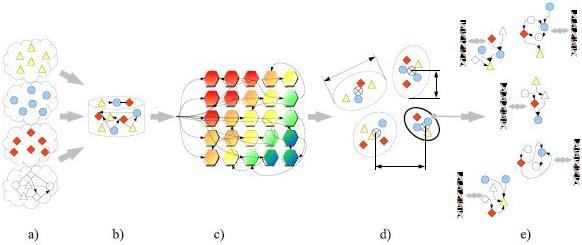
\includegraphics[scale=1.0]{{./fig1}.jpg}    
	    \caption{Enfoque basado en la inteligencia computacional para la minería de grandes datos en bioinformática:
    a) diferentes fuentes de datos biológicos; b) pre-procesamiento de los datos crudos, reducción, normalización e integración; c) clustering basado en mapas autoorganizativos y ensambles de agrupamientos; d) medidas de validación de las agrupaciones; e) metaheurísticas bioinspiradas para la inferencia de vías metabólicas y redes de regulación génica.}
    \label{fig:fig1}
\end{figure}
%%%%%%%%%


Investigadores del sinc(i) han propuesto recientemente una metodología general para la minería de datos biológicos en base a los paradigmas de la inteligencia computacional \cite{gsm2012}. Esta consta de una secuencia de tareas para integración y descubrimiento de conocimiento en datos biológicos. La secuencia incluye 5 pasos principales (Figura 1). El primer paso de la propuesta consiste en la obtención y especificación del tipo y número de fuentes de datos biológicos (Figura 1.a). El siguiente paso requiere la extracción de características relevantes y la integración de las diferentes fuentes de datos (Figura 1.b). La identificación de variaciones coordinadas en los datos se puede realizar mediante un modelo neuronal de tipo SOM (Figura 1.c) y otros métodos de clustering que mejoren la agrupación de los datos mediante la incorporación de una medida de similitud biológica durante el entrenamiento. La calidad de los clusters se mide en el siguiente paso  (Figura 1.d). El último paso de la propuesta consiste en el desarrollo de metaheurísticas bioinspiradas para el descubrimiento de nuevas vías metabólicas y redes de regulación a partir de las particiones identificadas en las etapas anteriores (Figura 1.e). Dentro de este esquema general se enmarca esta propuesta de tesis doctoral. En particular, en el paso de validación y medición de la calidad de las soluciones de clustering encontradas, se propone desarrollar índices que permitan estudiar las soluciones encontradas al aplicar algoritmos de clustering con diferentes parámetros y perturbaciones de los datos. 

Recientemente han surgido importantes aplicaciones y teorías que se orientan al análisis de soluciones con clusters solapados. Por ejemplo, en \cite{GoldbergHM10} se compara la evolución de grupos de personas en redes sociales y se propone un algoritmo para computar nuevas distancias entre colecciones de grupos potencialmente solapados. En esta tesis se propone realizar un análisis detallado de los índices existentes, mostrando las fallas que presentan ante soluciones con clusters solapados. A partir de esta revisión, se aplicará un enfoque probabilístico para desarrollar nuevos índices que puedan ser aplicables tanto a soluciones no solapadas como a soluciones solapadas. La propuesta a explorar gira fundamentalmente en torno a la idea de que las estimaciones de las probabilidades de encontrar dos o más objetos juntos en una u otra solución deben ser ajustadas teniendo en cuenta que hay objetos que pertenecen a más de un cluster en ambas soluciones. La propuesta de tesis incluye también la evaluación de una serie de propiedades básicas que debe cumplir un índice de este tipo. Además, deberá probarse su aplicabilidad en casos reales, demostrando claramente su superioridad ante condiciones de diverso grado de solapamiento y robustez ante la perturbación de los datos.

%-------------------------------------------
\subsection{Metodología general}
%-------------------------------------------
La metodología general a aplicar en el desarrollo de esta tesis consiste principalmente de ciclos que comprenden las siguientes etapas:
\begin{itemize}
	\item Actualización bibliográfica: estudio profundo de los conceptos y análisis de trabajos relacionados con el tema, de forma continua durante todo el desarrollo de la tesis. 
	\item Investigación exploratoria: análisis crítico de las principales propuestas disponibles actualmente para validación en clustering, que permitan ajustar la definición del problema y hacer propuestas de solución.
	\item Desarrollo e implementación computacional: de algoritmos de validación de clusters teniendo en cuenta criterios objetivos.
	\item Prueba de los métodos propuestos en esta tesis con datos sintéticos y en condiciones totalmente controladas.
	\item Diseño y experimentación numérica: prueba de los métodos propuestos, y comparación con los resultados obtenidos con otras técnicas del estado del arte aplicables a conjuntos de datos reales. 
	\item Publicación de resultados: a través de informes periódicos, reportes sobre los resultados obtenidos en las etapas anteriores y publicaciones científicas.
\end{itemize}


\subsection{Actividades}
\label{actividades}
Siguiendo la metodología general, 
en este plan de investigación se propone desarrollar medidas de validación que tengan en cuenta los puntos antes señalados, a partir de la ejecución de las siguientes actividades:
\begin{enumerate}
	\item Investigación bibliográfica.
	\item Generación de datos artificiales para experimentación, mediante diseño de métodos para 
agregado de ruido, re-muestreo y solapamiento de clusters.
	\item Estudio y análisis crítico de las propuestas existentes en cuanto a validación y estabilidad de soluciones.
	\item Propuesta de medidas para validación de agrupamientos considerando solapamiento en los agrupamientos.
	\item Experimentación numérica y prueba de los algoritmos con datos artificiales y reales.
	\item Implementación de formas de visualización de las salidas de los algoritmos.
	\item Publicación de resultados.
	\item Escritura del documento de tesis.
\end{enumerate}

%-------------------------------------------
\section{Grado de avance}
%-------------------------------------------
Al inicio de esta tesis se trabajó en el análisis y funcionamiento de algunos índices clásicos 
de validación externa. Paralelalente se exploraron alternativas para la generación artificial de datos que sirvan para la prueba de los índices creados. Se desarrolló una herramienta para la creación de grupos solapados, con la posibilidad de crear distintos grados de solapamiento y, de esta forma, poder verificar de forma controlada el comportamiento de los índices de validación.
De esta forma se entendió cómo trabajan las medidas más utilizadas, ya que existen varias que funcionan con distintos principios: los que cuentan de a pares de patrones, como Fowlkes-Mallows (FM)\cite{fowlkes_method_1983} y Jaccard (Jac)\cite{jac01}; los que cuentan la correspondencia que existe entre los clusters, como Maximum-Match (MM)\cite{meila_experimental_2001}; y por último están los  que se basan en teoría de la información y estadística, como el Normalized Mutual Information (NMI) \cite{vinh_information_2009}. Con dicho estudio, se logró comprender en qué medidas había una carencia de índices que se desempeñen correctamente en ciertas situaciones. Así, se detectó que los índices estudiados fracasaban
al momento de evaluar soluciones que se presentaban solapamiento. Es decir, soluciones en las 
que los patrones agrupados pueden pertenecer a más de un grupo.	De este modo, se diseñó inicialmente un índice
 que permite evaluar soluciones solapadas \cite{csm2014}. Si bien este
primer índice propuesto se desempeñó satisfactoriamente en las pruebas realizadas, luego se encontraron ciertas inconsistencias
a la hora de evaluar algunas soluciones. No obstante, este primer índice permitió explotar la naturaleza probabilística
del conteo de pares de patrones para la evaluación de soluciones solapadas. Con esto se abrió camino
a la creación de un nuevo índice, Overlapped Clusters ($\mathcal{OC}$)\cite{csm2016}. 
Este índice, trabaja con un par de soluciones de clustering a comparar: $C$ y $C^\prime$, con 
$k$ y $k^\prime$ grupos, respectivamente. De esta forma, $c_i$ ($c^\prime_j$), representa al cluster $i$ ($j$) de la solución $C$ ($C^\prime$).
La la cantidad de patrones del conjunto de datos es $N$. Con $n$ y $n^\prime$ se indica la cantidad de patrones que se llegan a contar en los grupos de $C$ y $C^\prime$, teniendo en cuenta el solapamiento de los mismos.
Luego, el índice propuesto se definió como

\begin{equation}
	\mathcal{OC} = \frac
		{\tilde{t}}
		{\max(\tilde{p},\tilde{p}^\prime)},
	\label{final:formula}
\end{equation}

\noindent donde 

\begin{equation}
	\tilde{t} = \frac
		{\sum\limits_{i=1}^{k} 
			\sum\limits_{j=1}^{k^{\prime}} \binom{\left|c_i \cap c_j^{\prime}\right|}{2}}
		{\binom{N}{2} \frac{\max(n, n^{\prime})}{N} \min(k,k^{\prime})}
	\label{newotk}
\end{equation}

\noindent y

\begin{equation}
	\tilde{p} = \frac{\sum\limits_{i=1}^{k} \binom{\left|c_i\right|}{2}}
					{k\binom{N}{2}},
	\label{newopk}
\end{equation}

\noindent siendo $\tilde{p}$ una estimación de la probabilidad de encontrar un par de elementos juntos en cualquier clúster $c_i$ de $C$. De la misma manera sucede con $\tilde{p^\prime}$ para cualquier cluster $c^\prime_j$ de $C^\prime$. En (\ref{newotk}), $\tilde{t}$ representa la probabilidad de que un par de patrones se agrupen juntos en ambas soluciones. 
De esta forma $\mathcal{OC}$ puede ser definido como la razón entre la probabilidad de encontrar dos patrones juntos en ambas soluciones y la máxima probabilidad de encontrarlos en una del ellas.


El índice propuesto se mostró sólido en distintas pruebas con clusters solapados. Tanto en tests artificiales pero extremos en cuanto a valores esperados, como en datasets reales. Con respecto a estos últimos, se hicieron pruebas sobre bases de datos bien conocidas: Iris, Wine, Yeast y Glass\footnote{\url{http://archive.ics.uci.edu/ml/datasets/}}. A cada uno de estos datasets se le aplicó un particionamiento usando SOM. Debido a que cada neurona de un mapa puede tomarse como un cluster, y considerando que neuronas vecinas del mapa agrupan datos similares, fue sencillo probar distintos grados de solapamiento utilizando este hecho. 
Por ejemplo, en el Cuadro 1 %\ref{table:datasets} 
se puede observar una de las pruebas realizadas, sobre la base de datos Iris (el mismo experimento se realizó en las mencionadas con similares resultados). En la columna 1 se observa el nombre del conjunto de datos, en la columna 2 se observa el número de clusters considerados en $C$ y en $C^\prime$, y en las columnas 3--6 se puede observar el valor arrojado para cada índice y experimento considerado. Cada una de las últimas 4 columnas se dividió en 2, para considerar el experimento sin solapamiento ($V_n=0$, donde $V_n$ significa vecindad entre neuronas del SOM) y con solapamiento ($V_n=1$) en la solución $C^\prime$. 

También se realizó una prueba en un conjunto de datos reales, correspondientes a una red social (YouTube)\cite{yang_defining_2013}. En el mismo se tomó un conjunto de datos que poseía varios grupos con 2 ó más usuarios que compartían intereses en común. A cada grupo se lo definió como una comunidad. Cada usuario puede tener varios intereses y pertenecer a más de una comunidad. De esta forma, se tiene un típico particionamiento solapado. El nivel de solapamiento de una comunidad depende del número de participantes que se encuentran también en otras comunidades. El experimento consistió en ordenar el conjunto de datos por nivel de solapamiento. Con esto se conformaron las soluciones de referencia ($C$).  
A partir de las mismas, se formaron las soluciones ($C^\prime$) a las que se les aplicó un 20\% de perturbaciones aleatorias, añadiéndo usuarios a algunas comunidades. Luego, se dividió cada conjunto de datos en 17 subconjuntos, que se fueron comparando de a pares con los índices FM y $\mathcal{OC}$. Con esto, los resultados obtenidos indicaron que, a medida que el grado de solapamiento era mayor, el índice propuesto se mantenía prácticamente estable, marcando el grado de perturbación del dataset pero siendo inmune al solapamiento. Por otro lado, el índice FM mostró una tendencia a decrecer a medida que aumentaba el solapamiento. Estos resultados se enviaron a la revista Expert Systems with Applications (Elsevier), de Factor de Impacto 2,240 (año 2014).


%%%%%%%%%
% Table 4
\begin{table}
\begin{scriptsize}
\caption{Resultados para los índices FM, ARI, JAC y {{\paperindex}}, sobre particiones de la base de datos Iris.
		La solución de referencia $C$ posee $4$ o $25$ clusters sin solapamiento. 
		Las soluciones $C^{\prime}$ tiene $25$ y $100$ clusters,
		con y sin solapamiento.}
\end{scriptsize}
\label{table:datasets}
\begin{center}
	\begin{scriptsize}
		\begin{tabular}{c | c | c | c | c | c | c | c | c | c }
		\hline\noalign{\smallskip}
		  \multirow{2}{*}{} & \multirow{2}{*} { \textbf{clusters en $C$ y $C^\prime$}} & \multicolumn{2}{c|}{\textbf{FM}} & 	\multicolumn{2}{c|}{\textbf{ARI}} &	\multicolumn{2}{c|}{\textbf{JAC}} &	\multicolumn{2}{c}{\textbf{\paperindex}}\\
         & & \textbf{$Vn=0$} & \textbf{$Vn=1$}  & \textbf{$Vn=0$} & \textbf{$Vn=1$} & \textbf{$Vn=0$} & \textbf{$Vn=1$}& \textbf{$Vn=0$} & \textbf{$Vn=1$}\\
		\noalign{\smallskip}\hline\noalign{\smallskip}		
        \multicolumn{5}{c}{} \\ %
        \multirow{3}{*}{Iris} & $k=4$ vs $k^{\prime}=25$  &   $0.33$ & $0.30$ & $0.16$ & $4.26 $ & $0.14$ & $0.10$& $0.14$& $0.38$ \\
        &$k=4$ vs $k^{\prime}=100$  &  $ 0.17  $  & $ 0.16$  & $ 0.03$ & $-0.66$& $0.03$& $0.03$& $0.03$& $0.11$\\
        \cdashline{2-10}[0.5pt/1pt]
        &$k=25$ vs $k^{\prime}=100$  & $ 0.33$  & $	0.23 $  & $ 0.23 	 $ & $	-0.34$ & $0.14$& $0.09$& $0.14$& $0.37$\\
        \hline\hline
		\end{tabular}		
	\end{scriptsize}		
\end{center}
\end{table}
%%%%%%%%%


Con respecto a las actividades propuestas en esta tesis de doctorado, estarían faltando las  relacionadas con los ítems 6  y 8 de la Sección \ref{actividades} (``Implementación de formas de visualización de las salidas de los algoritmos'' y  ``Escritura del documento de tesis'').
%-------------------------------------------
\section{Factibilidad}
%-------------------------------------------
El doctorando tiene a disposición el equipamiento e instalaciones del Centro de Investigación y Desarrollo en Ingeniería en Sistemas de Información (CIDISI--FRSF--UTN). Además, el candidato cuenta con el Instituto de Investigación en Señales e Inteligencia Computacional (sinc(\emph{i})), donde desempeña sus actividades de investigación el director y co-director propuesto, Dra. G. Stegmayer y Dr. D. Milone, respectivamente. Desde este Instituto se posee acceso a un cluster de 50 computadoras que será utilizado fundamentalmente para los experimentos numéricos de la tesis, dada la gran cantidad de datos a procesar y el costo computacional de los algoritmos de validación. 

Los recursos financieros con los que se contará para realizar las tareas propuestas provendrán de los siguientes proyectos: PIP CONICET 117: \textit{Minería de datos en bioinformática: un enfoque integrado basado en la inteligencia computacional}, director: G. Stegmayer; PICT 2014-2627: \textit{Minería de datos en bioinformática: integración y análisis basados en inteligencia computacional}, director: D. Milone y CAI+D 548: \textit{Modelos y algoritmos para minería de datos en bioinformática}, director: G. Stegmayer.
Los datos para la experimentación están disponibles en forma gratuita en Internet.


%-------------------------------------------
\bibliographystyle{splncs}
\bibliography{prop_tesis}
\end{document}